\Chapter{Risk Aware Exploration}\label{sec:Theme2}

In this chapter, the article in which \ac{DORA} was first described \cite{vielfaure2021dora} is summarized. \ac{DORA} was created in the context of this thesis and is closely related to the theme of risk awareness in swarm robotics. To avoid redundancy and to make this chapter more concise, the related works and background necessary to understand this system are presented in Ch. \ref{sec:RevLitt}. Figures in this chapter are taken from the article with permission from the authors.

Because exploration of unknown environments is an important challenge in the
field of robotics, we wanted to show the benefits of taking risk awareness into account when developing solutions for this kind of challenge. We based our exploration strategy on distributed belief maps. This way, swarm efficiency is leveraged because robots collaborate by sharing useful information. The key idea behind \ac{DORA} is to minimize risk exposure while maximizing exploration coverage, leading to more efficient exploration because of fewer risk-related failures. 


\section{Introduction}
Unknown environment exploration by robots has applications in numerous fields. For example, search-and-rescue missions \cite{matos2016multiple} and space missions \cite{fong2005interaction} can both benefit from using robots, as they often operate in environments inaccessible to humans. This inaccessibility can stem from multiple causes, such as the remote nature of these places (space, other planets, oceanic depths), the impossibility for humans to reach them (caverns with too small openings) or their dangerous nature (radioactive zones, forest fires, flooded areas). For all of these, there is necessarily an associated risk factor, which means that robots sent to explore them will necessarily be exposed to some danger increasing the risk of failures. Robot swarms mitigate the effects of individual failures ~\cite{ramachandran2019resilience,wehbe2021probabilistic,winfield2006safety} and improve overall terrain coverage performance \cite{burgard2005coordinated}. However, even in robot teams, failures have negative effects on overall performance, which is why we sought to reduce them as much as possible through \ac{DORA}.

The motivation for creating a purely decentralized algorithm is to avoid the pitfalls related to centralized systems, such as bottlenecks and single points of failures. The first can be related to low capacity robots, or to noisy environments affecting communication efficiency or causing memory corruption. The second is particularly important in the risky scenarios where individual malfunctions are more likely and could cause system-wide failures. Consequently, relying on locally shared information and onboard computation is necessary.

As we found no existing decentralized risk-aware exploration algorithm, we sought to create one.


\section{System Model}
\label{dora_system_model}

The motivation for including risk awareness in a distributed exploration algorithm can be seen in Fig. \ref{risk_unaware}, where failures lead to decreasing performance over time. Conversely, in Fig. \ref{risk_aware}, avoiding dangerous areas reduces failures and maintains exploration efficiency. In order to design our system, we modelled the environment as a 2D grid ($E \subset \mathbb{Z}^2$) in which agents $a_i \in A$ carry out their task. Several design considerations shaped \ac{DORA}. They are summarized here, and more details can be found in the referenced paper.

\FloatBarrier

First, risk and failure probability had to be formally modelled. We chose to represent risk as point radiation sources $s_j \in S$ with an exponentially decaying intensity $I_j$, but any other type of danger could have been used with our system. The equations representing the radiation perceived by a robot $a_i$ failing due to radiation in cell $\bm{x}_i$ can be combined as:

\begin{equation}
    r(\bm{x}_i) = b + \sum_{\bm{s}_j \in S} \frac{I_j}{1 + \lambda\rho_j^2}
    \label{eq:radiation_dora}
\end{equation}

Where $\rho_j$ is the distance between $a_i$ and $s_j$, $\lambda$ is a decay constant and $b$ is Gaussian noise. The probability of failure necessarily increases where $r(\bm{x}_i)$ is higher.

Second, we defined the objective of exploration as gaining information by visiting cells from $E$. Logically, recently visited cells are unlikely to yield any information gain. Therefore, priority is given to unvisited and less recently visited cells. Doing so requires saving the last time of exploration of $\bm{x}_i$ in a scalar field $\epsilon(\bm{x}_i) = t_\epsilon$. The probability of finding useful information decreases exponentially for values of $\epsilon(\bm{x}_i)$ which are closer to the current time step $t$.

Third, as way of storing these values, we use a \ac{CRDT}: the virtual stigmergy from \cite{pinciroliTuple2016}. This allows robots to exchange information whenever possible (thereby achieving a loose eventual consistency) without relying on a central communication hub. Both $r(\bm{x}_i)$ and $\epsilon(\bm{x}_i)$ are stored in distributed belief maps. These are updated at every time step.

Fourth, we describe a position-based control law for the robots which minimize risk and maximize information gain. These optimizations are described by local gradients of each scalar field in a Moore neighborhood (see Fig. \ref{neighborhood}) around $a_i$.

\begin{figure}[htbp]
	\centering
    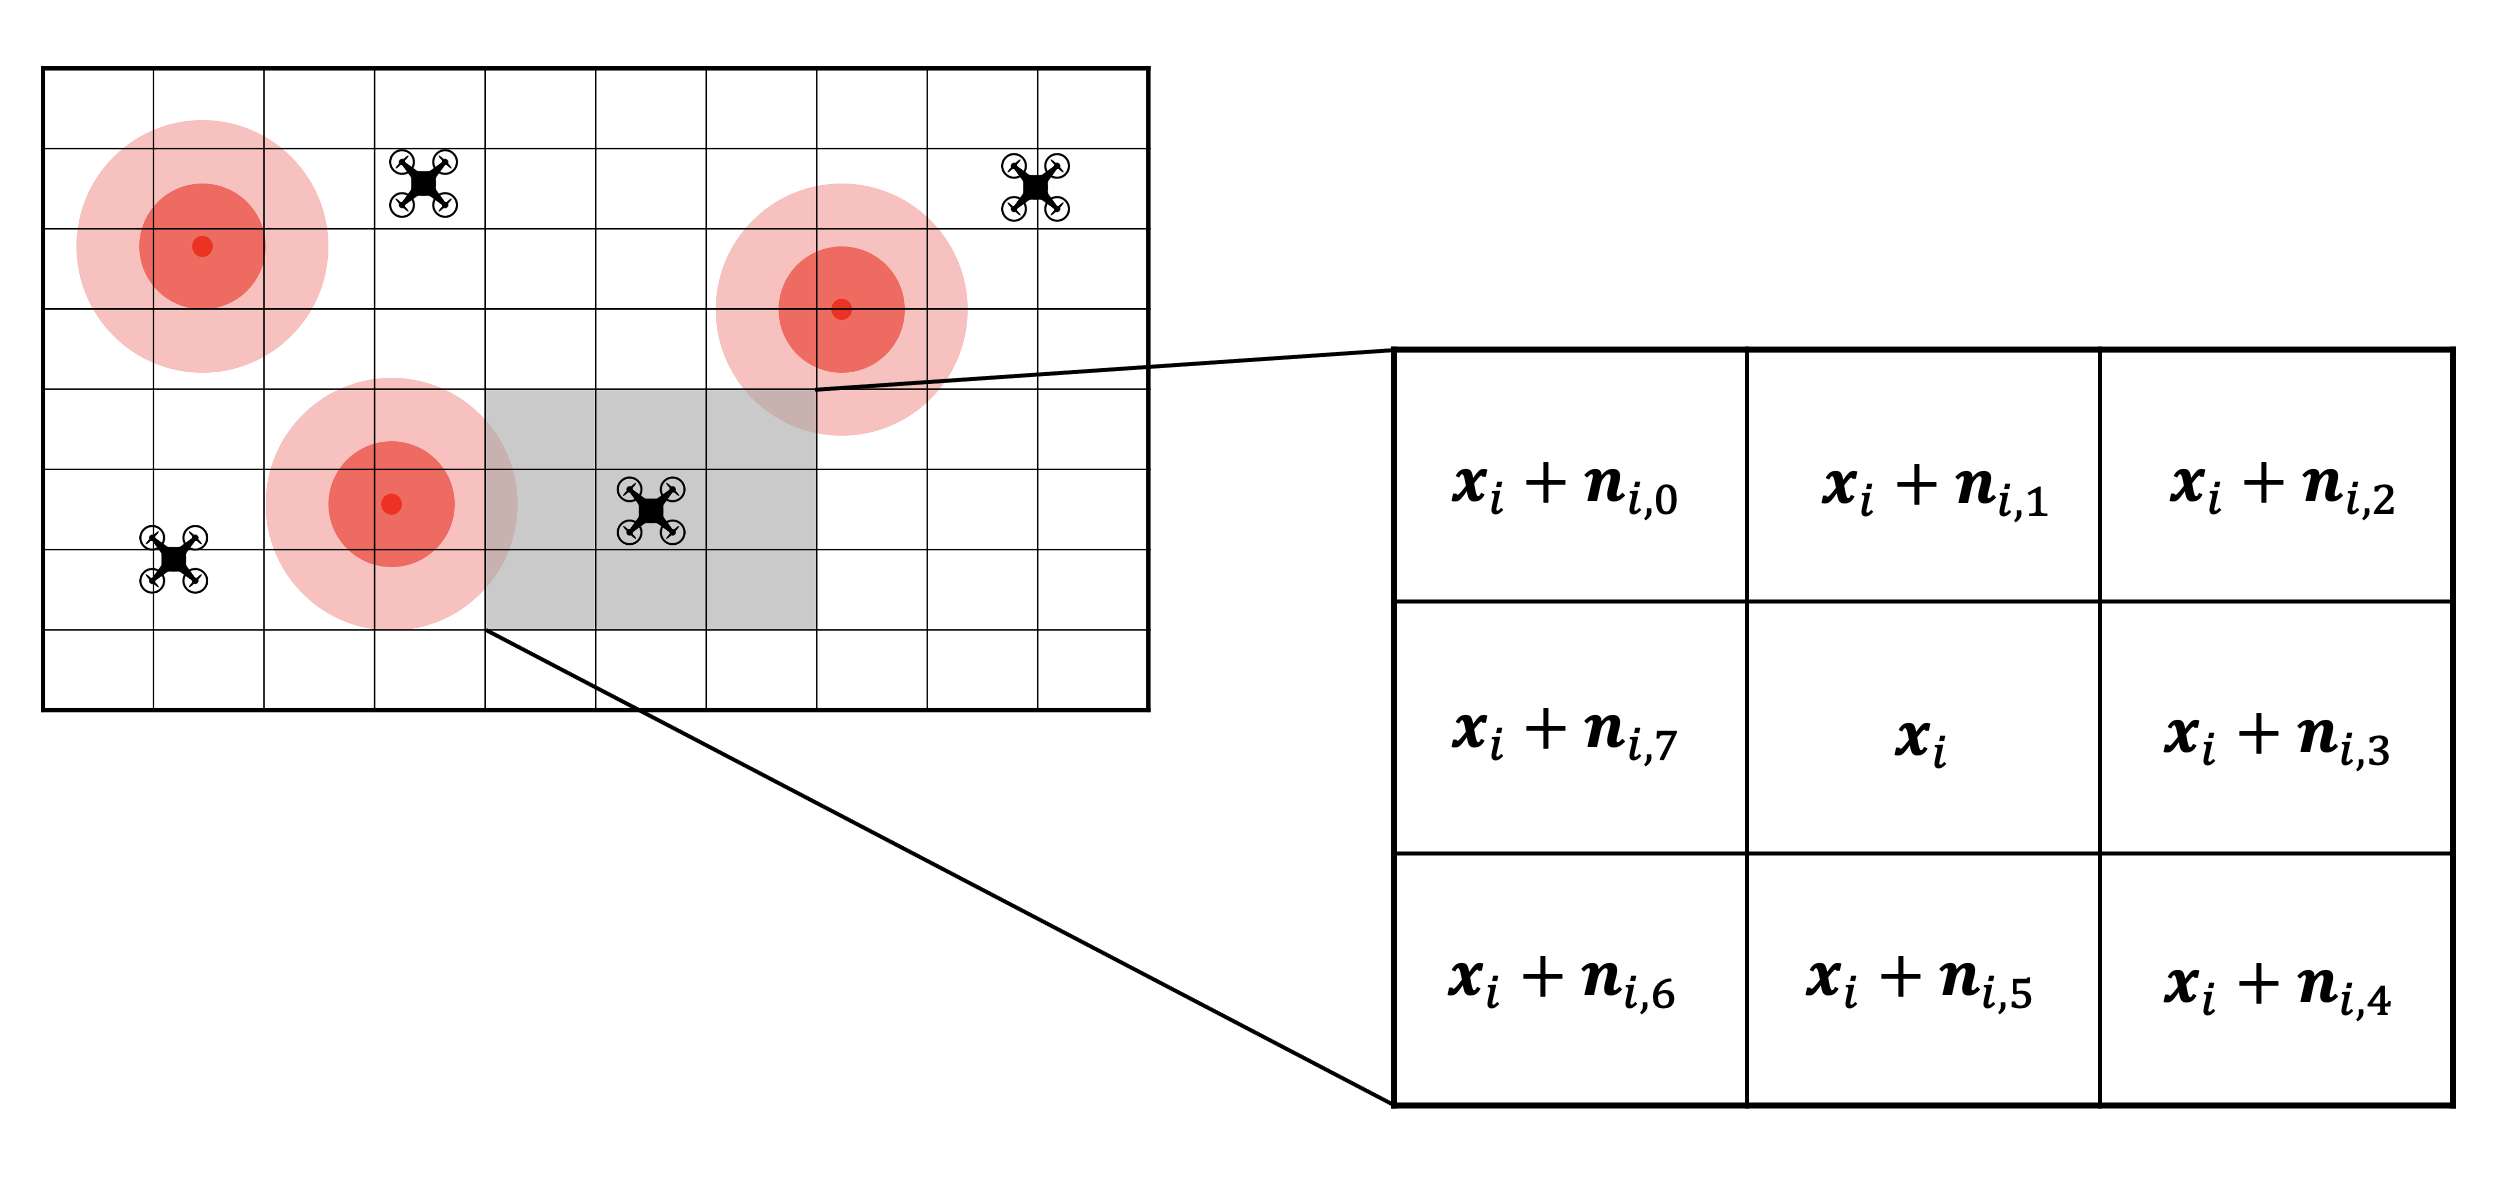
\includegraphics[width=0.95\columnwidth]{figures/dora_explorer/Moore.png}
    \caption[Moore neighborhood]{$\bm{x}_i$'s neighborhood. $\bm{n}_{i,0} = (-1, 1)$ is neighbor 0's offset from $\bm{x}_i$.}
    \label{neighborhood}
\end{figure}

The risk gradient $\bm{\nabla}_{r;i}$ is given by:

\begin{equation}
    \bm{\nabla}_{r;i} = \sum_{\bm{n}_j \in \nu}\bm{\hat{n}}_{i,j} \cdot (r(\bm{x}_i) - r(\bm{n}_{i,j}))
    \label{eq:gradient}
\end{equation}

where $\bm{\hat{n}}$ is the unit form of $\bm{n}$. The exploration gradient $\bm{\nabla}_{\epsilon;i}$ is calculated in the same manner. We combine these to obtain the control law:

\begin{equation}
    \bm{x}_i^{t+1} = \bm{x}_i^t + (\alpha\bm{\nabla}_{r;i} + \beta\bm{\nabla}_{\epsilon;i} + \gamma\bm{o}_i)
    \label{eq:control_law}
\end{equation}

where $\alpha, \beta, \gamma$ are parameters related to risk avoidance, exploration gain and obstacle avoidance control. The latter is added from robustness and inspired from \cite{shahriari2018lightweight}.

\begin{figure*}
     \centering
     \begin{subfigure}{0.45\textwidth}
         \centering
         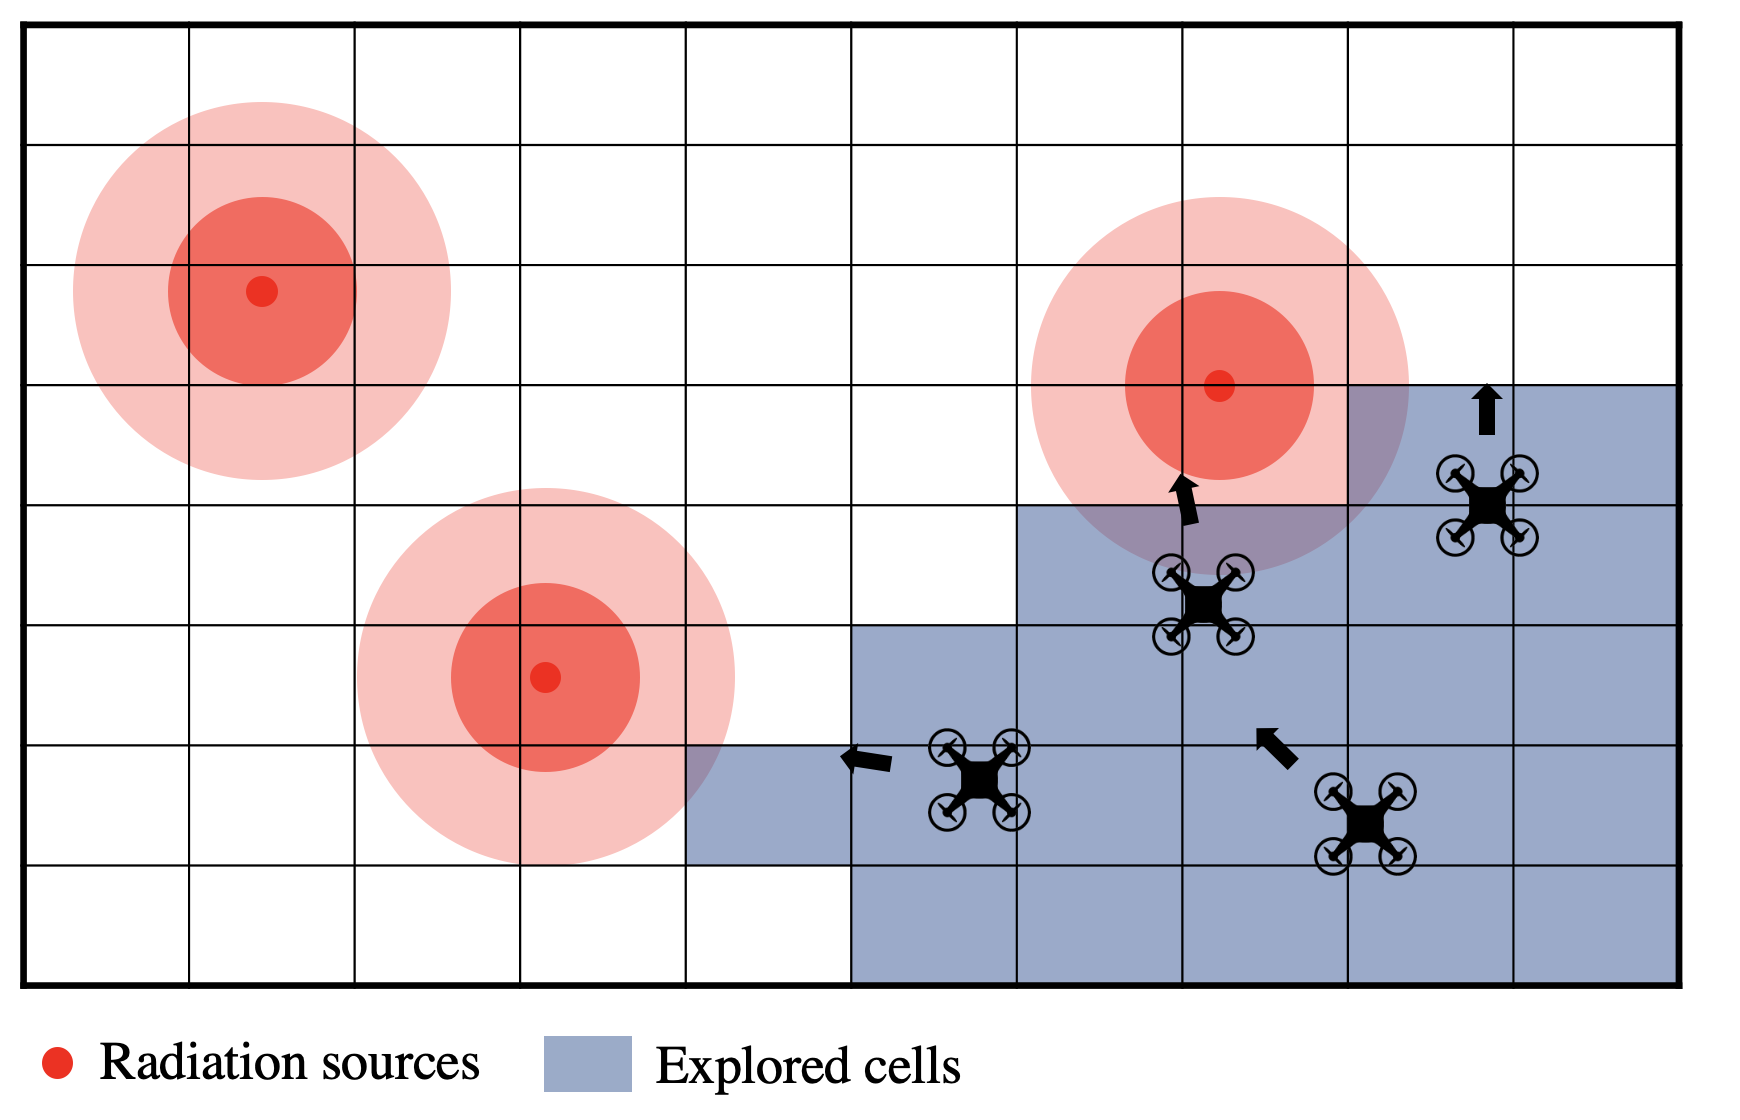
\includegraphics[width=\textwidth]{figures/dora_explorer/risk_aware_b.png}
         \caption{}
         \label{risk_unaware_a}
     \end{subfigure}
     \begin{subfigure}{0.45\textwidth}
         \centering
         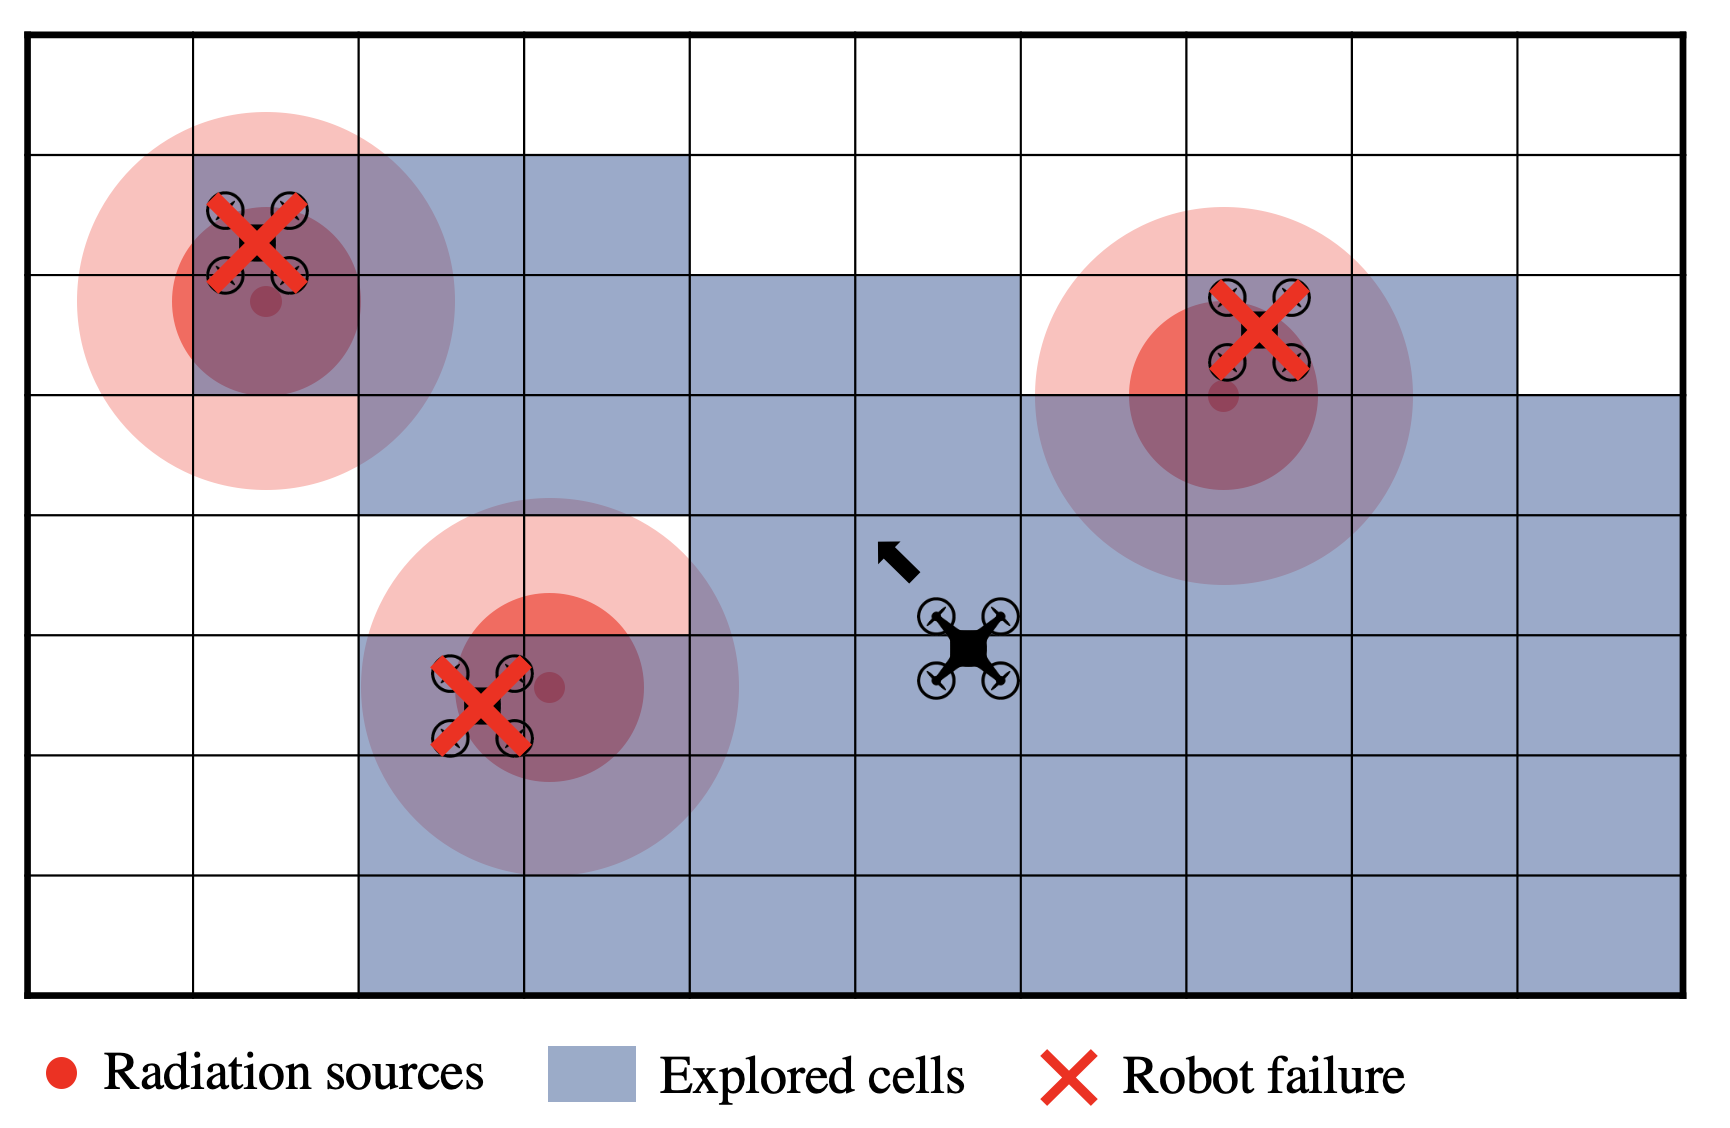
\includegraphics[width=\textwidth]{figures/dora_explorer/risk_unaware_a.png}
         \caption{}
         \label{risk_unaware_b}
     \end{subfigure}
        \caption[Risk-unaware exploration intuition]{Exploration without risk awareness. Fig. \ref{risk_unaware_a}: Robots start exploring but are unable to sense environmental radiation. The only driving force of the algorithm is exploring new cells. Fig. \ref{risk_unaware_b}: Robots fail because they do not discriminate between safe and dangerous cells. Exploration is carried out by fewer robots. Exploration efficiency drastically decreases and large areas of the environment remain uncovered.}
        \label{risk_unaware}
\end{figure*}

\begin{figure*}[htbp]
    \centering
    \begin{subfigure}{0.45\textwidth}
         \centering
         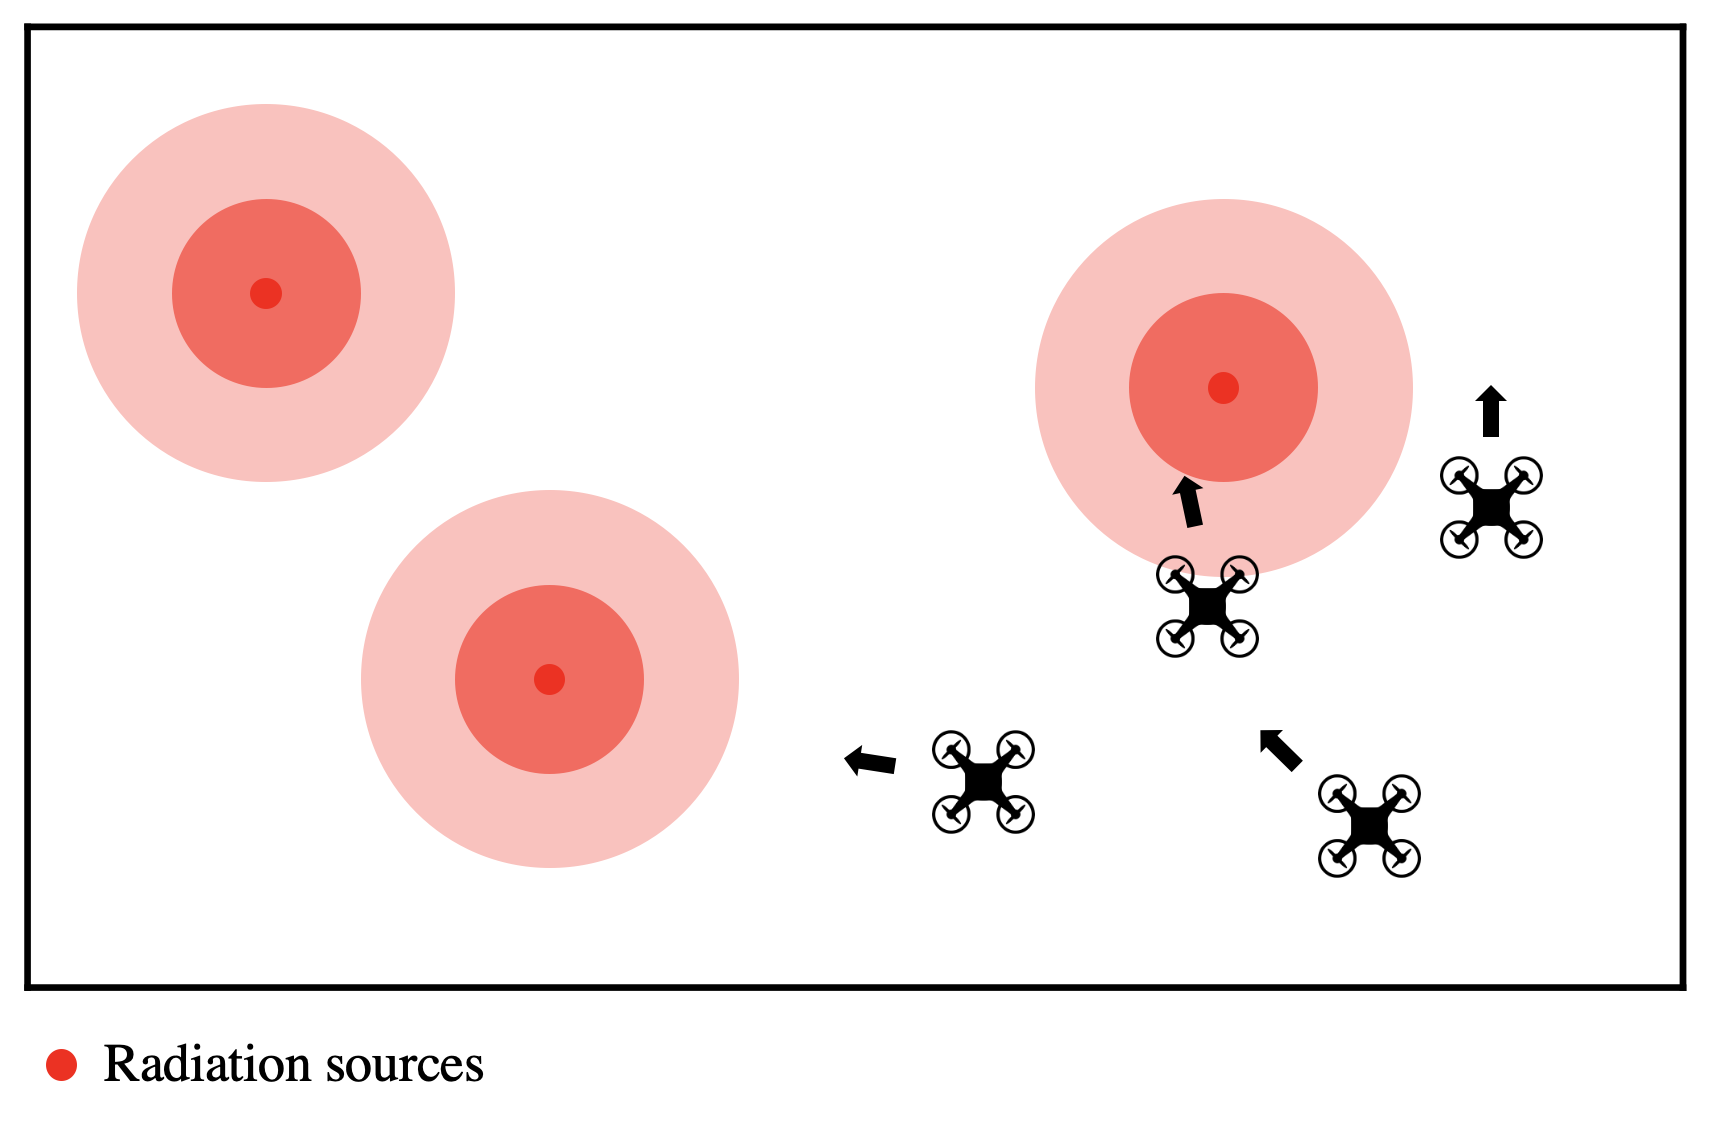
\includegraphics[width=\textwidth]{figures/dora_explorer/risk_aware_a.png}
         \caption{}
         \label{risk_aware_a}
    \end{subfigure}
    \begin{subfigure}{0.45\textwidth}
         \centering
         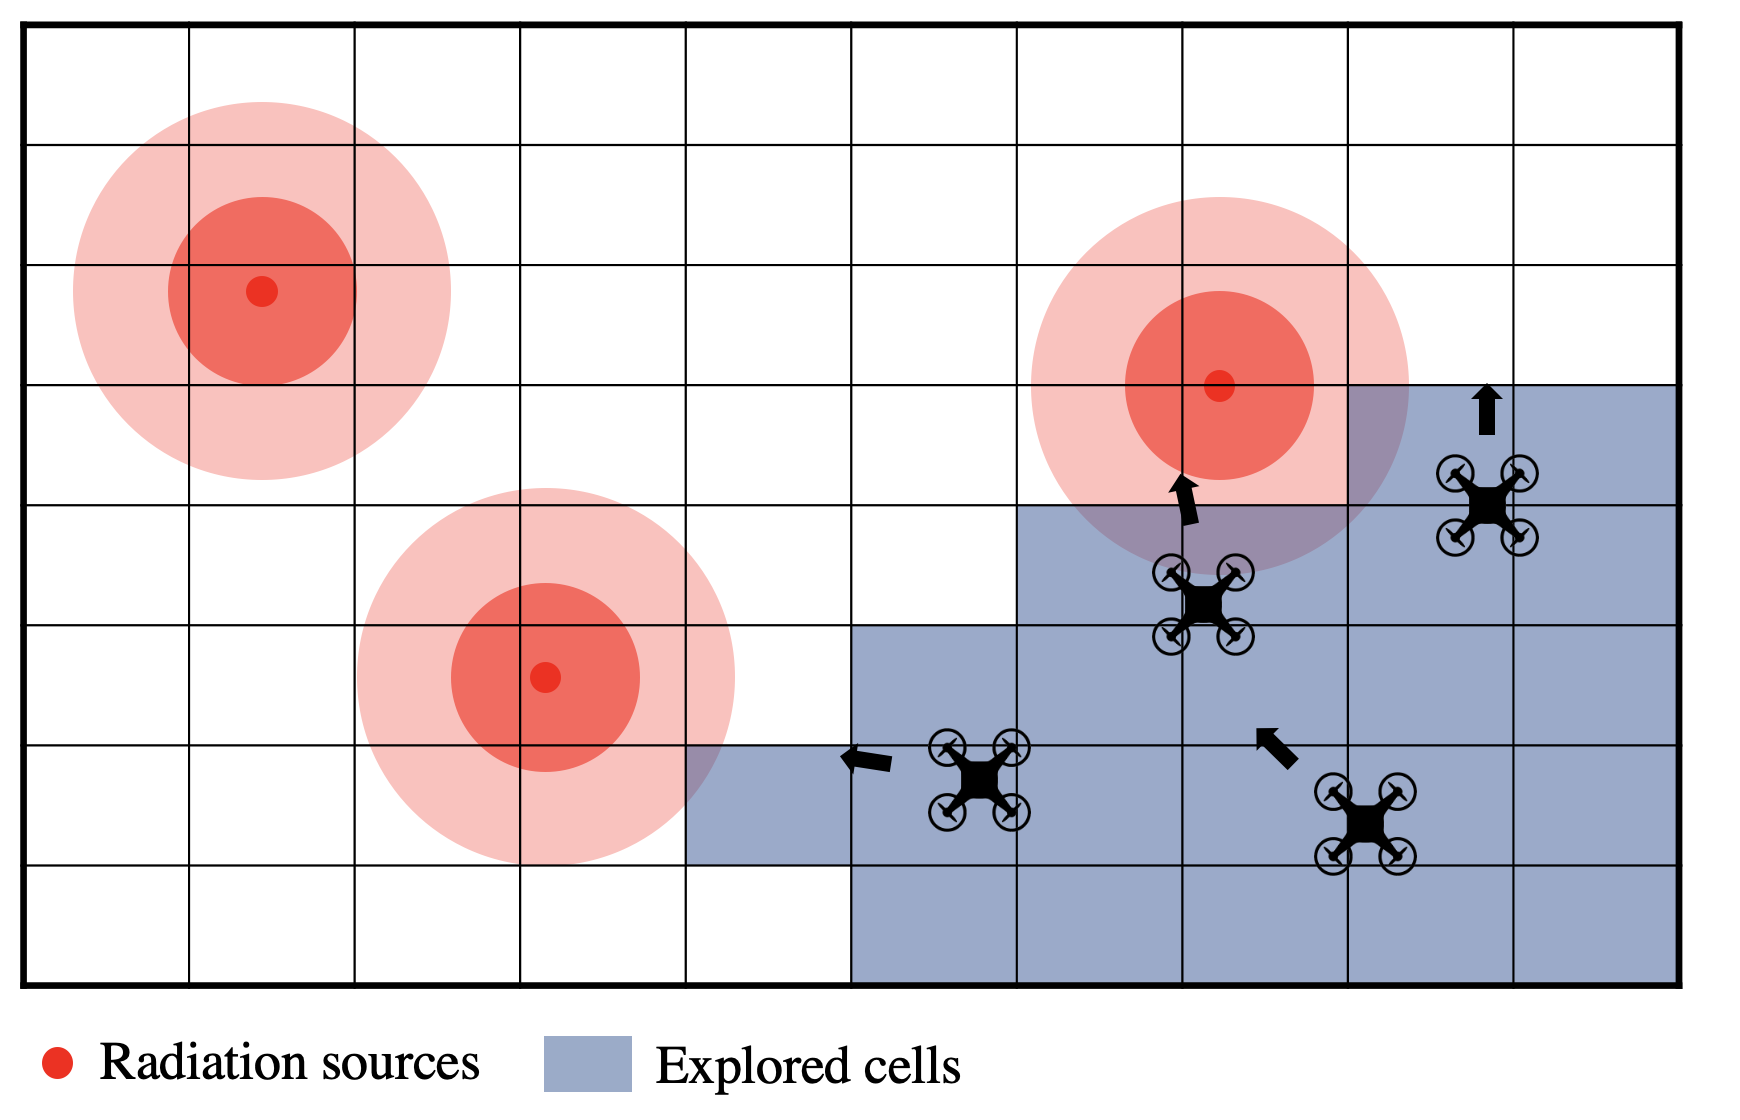
\includegraphics[width=\textwidth]{figures/dora_explorer/risk_aware_b.png}
         \caption{}
         \label{risk_aware_b}
    \end{subfigure}
    \begin{subfigure}{0.45\textwidth}
         \centering
         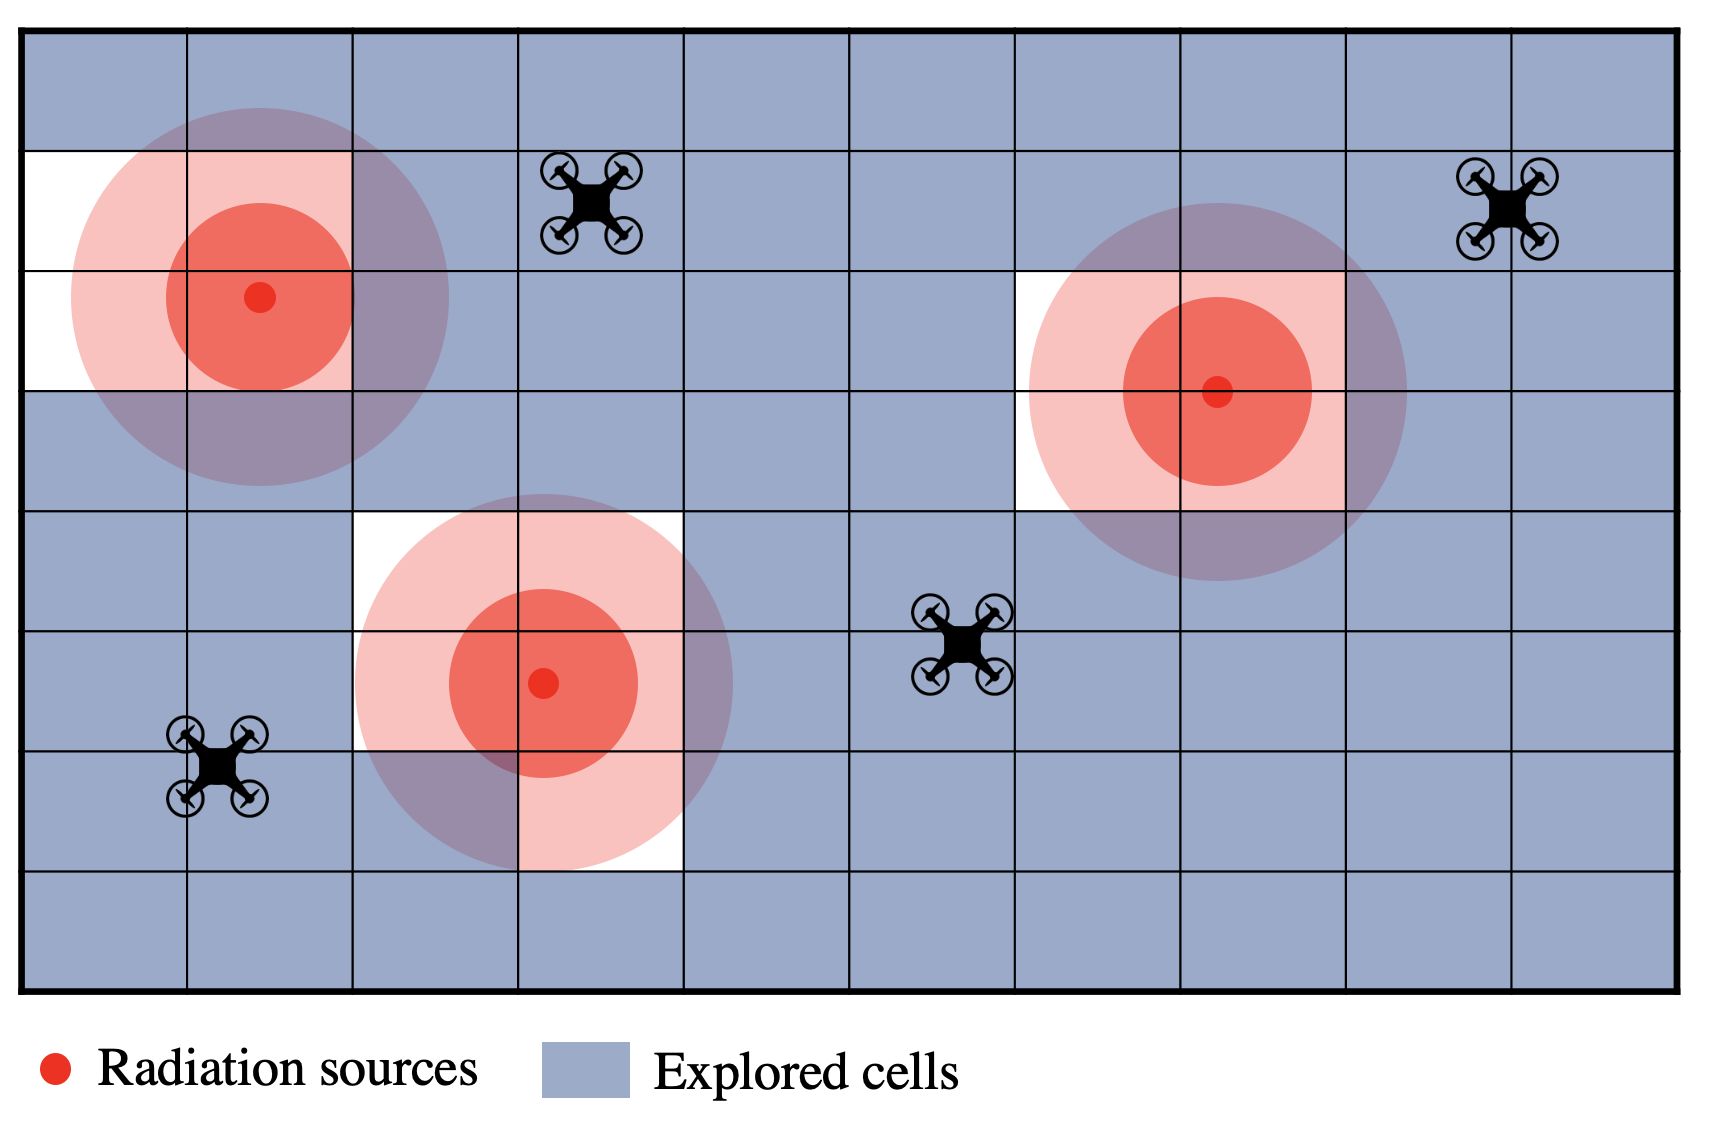
\includegraphics[width=\textwidth]{figures/dora_explorer/risk_aware_c.png}
         \caption{}
         \label{risk_aware_c}
    \end{subfigure}
    \begin{subfigure}{0.45\textwidth}
         \centering
         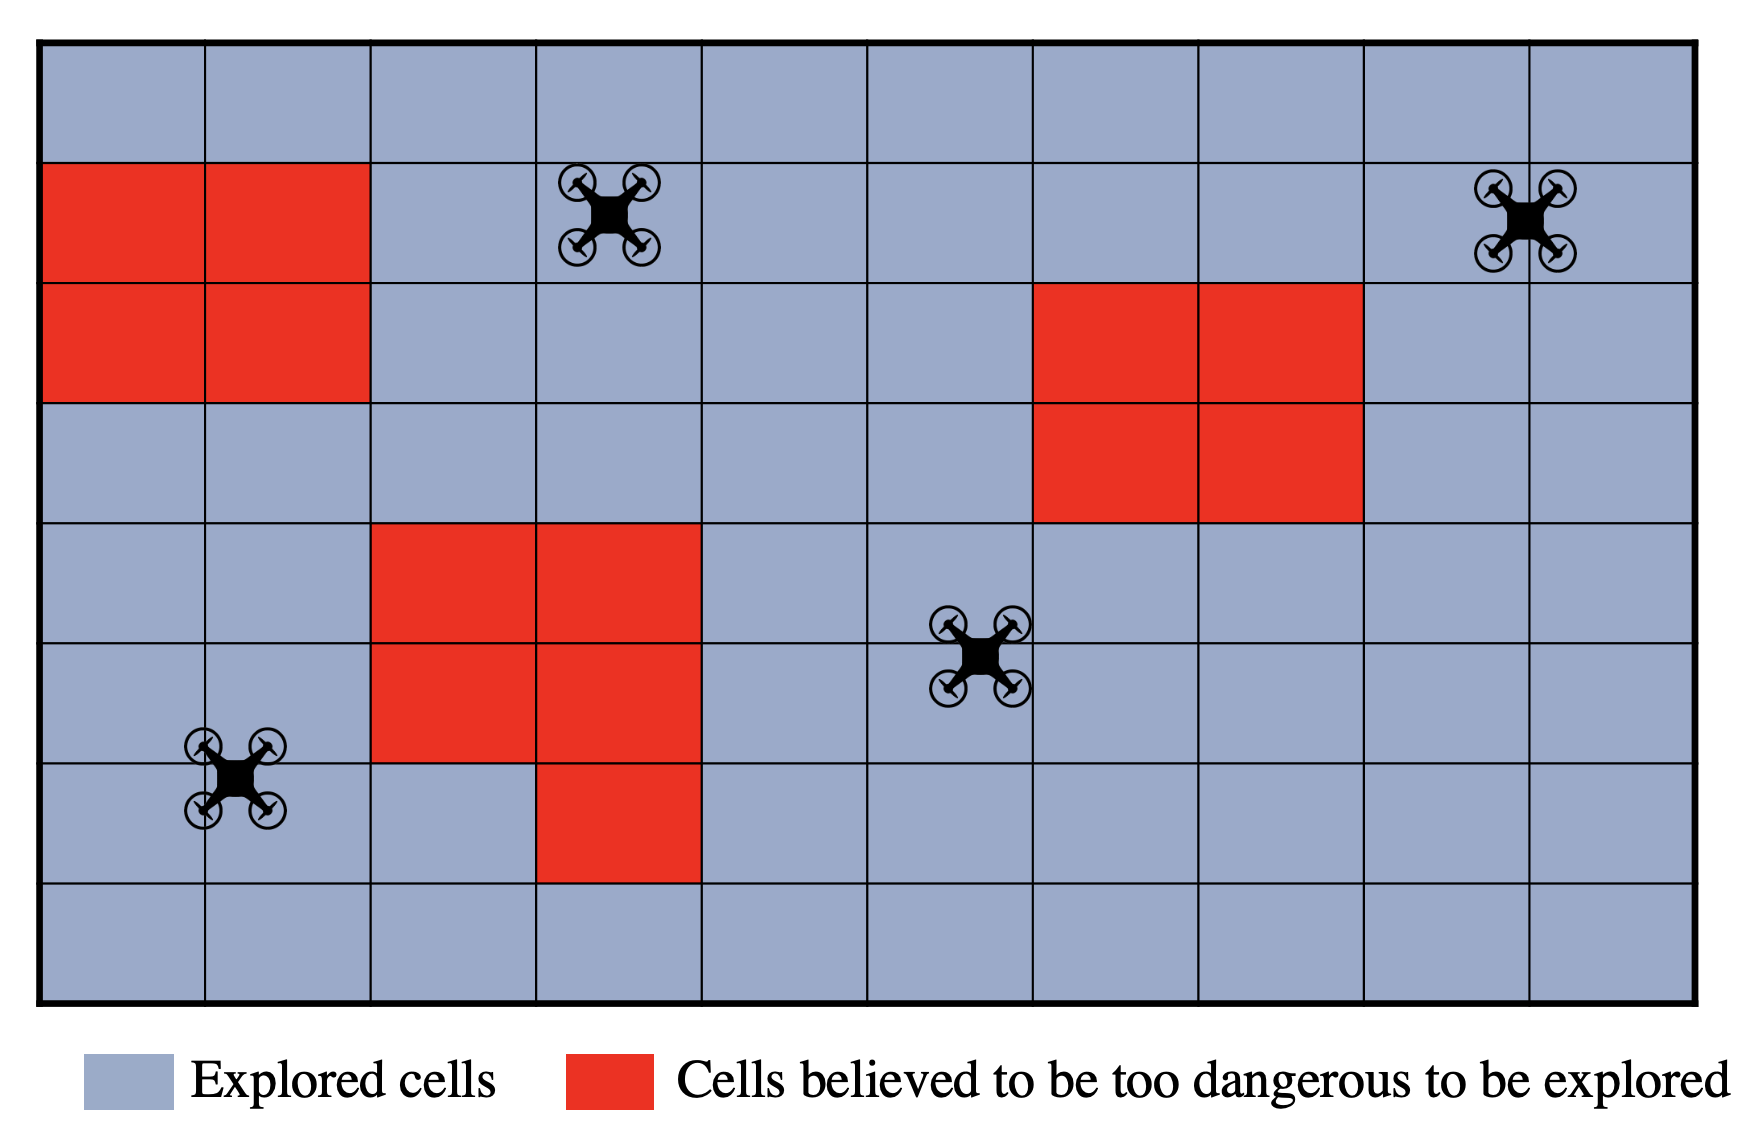
\includegraphics[width=\textwidth]{figures/dora_explorer/risk_aware_d.png}
         \caption{}
         \label{risk_aware_d}
    \end{subfigure}
        \caption[Risk-aware exploration intuition]{Risk aware exploration intuition. Fig. \ref{risk_aware_a}: Robots start exploring a hazardous environment. Fig. \ref{risk_aware_b}: A grid is formed. When a new cell from this grid is explored, the sensed radiation is used to update the \ac{DBM}. Fig. \ref{risk_aware_c}: The cells have been mostly covered by the robots. Fig. \ref{risk_aware_d}: Only cells believed to be too dangerous remain unexplored.}
    \label{risk_aware}
\end{figure*}

Finally, to ensure scalability, we made sure \ac{DORA}'s computational and communication costs remained low. They are represented by $C(A, \nu, E)$ and $D(A, \nu, E)$ where $\nu$ is the neighborhood and they are both bounded by $\Theta(|\nu|)$ because of the nature of the algorithm and of the virtual stigmergy.

\section{Experiments}
We performed experiments both in simulations and on physical robots. In both cases, for consistency, we used KheperaIV \cite{kteam2021kheperaiv} robots, which are relatively small and equipped with infrared sensors required for obstacle avoidance. It should be noted that they are capable of wireless networking through the 802.11b/g WiFi protocol, making swarm communication possible. We compared our algorithm with two baselines: \ac{FBE} and a random walk algorithm. The metrics we used to evaluate our system's performance were the number of active (not failed) robots over time, the total number of cells explored over time, and the bandwidth usage. Failures were triggered randomly based on (emulated) perceived radiation from \eqref{eq:radiation_dora}. Detailed motivation for parameter and metric choices can be found in the article.

The first step was to test \ac{DORA} by doing simulations in ARGoS. To verify the effect of swarm size on scalability, we ran our virtual experiments with varying swarm sizes ($N =\{10, 15, 20\}$) deployed randomly in a 20x20m environment with randomly positioned radiation sources and obstacles. To be thorough, we performed 50 simulation runs with 300 time steps each for each algorithm. 

The second step was the physical experiments. We ran them on 5 robots with fewer time steps (200) because of equipment and time constraints respectively. Robot positioning was obtained through motion tracking performed with OptiTrack Motive \cite{optitrack2021motive}. The environment consisted of a 2x2m arena split into a 10x10 cell grid.

\FloatBarrier

\section{Results}
The following shows the average results obtained in the simulation runs as well as those from physical experiment runs.

Fig. \ref{results:dora_explored} shows that \ac{DORA} attains similar terrain coverage to \ac{FBE}. Moreover, the performance gap between the two reduces as $N$ increases, showing good scalability from \ac{DORA}. Both algorithms outperform the random walk one by far. Interestingly, \ac{DORA} covered more cells than \ac{FBE} in physical experiments. This is probably because the small size of the arena presented a pathological case for \ac{FBE}. 

\begin{figure*}
    \centering
    \begin{subfigure}{0.45\textwidth}
        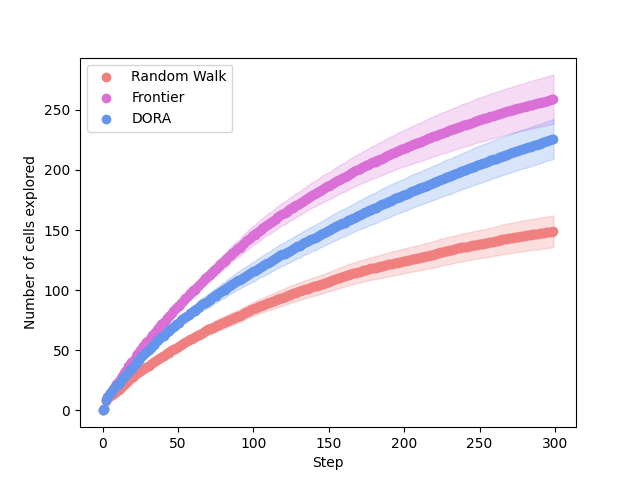
\includegraphics[width=\textwidth]{figures/dora_explorer/explored_10.png}
        \caption{N=10 robots}
        \label{results:explored10}
    \end{subfigure}
    \begin{subfigure}{0.45\textwidth}
        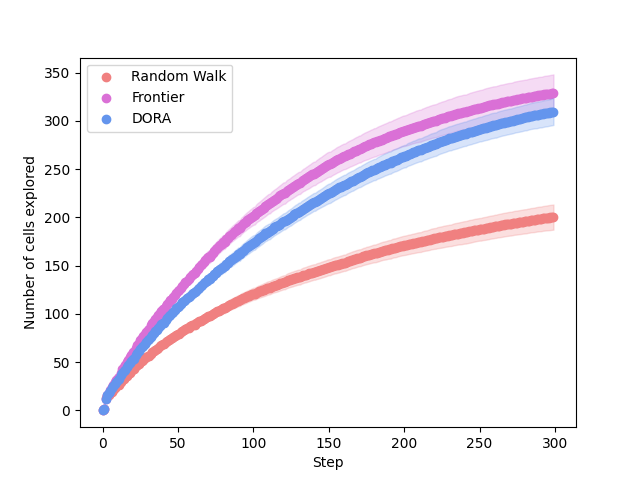
\includegraphics[width=\textwidth]{figures/dora_explorer/explored_15.png}
        \caption{N=15 robots}
        \label{results:explored15}
    \end{subfigure}
    \begin{subfigure}{0.45\textwidth}
        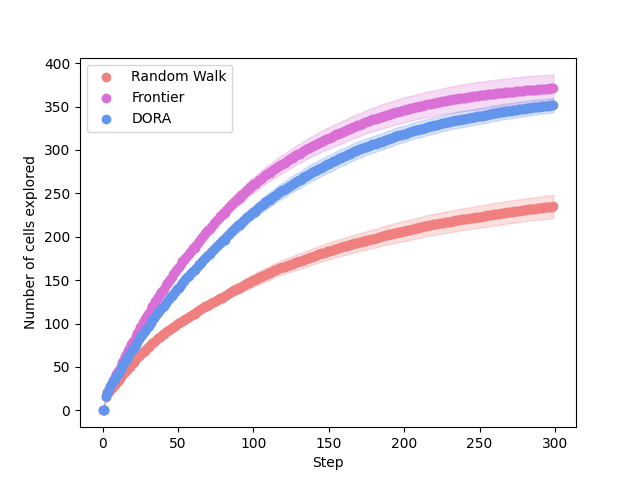
\includegraphics[width=\textwidth]{figures/dora_explorer/explored_20.png}
        \caption{N=20 robots}
        \label{results:explored20}
    \end{subfigure}
    \begin{subfigure}{0.45\textwidth}
        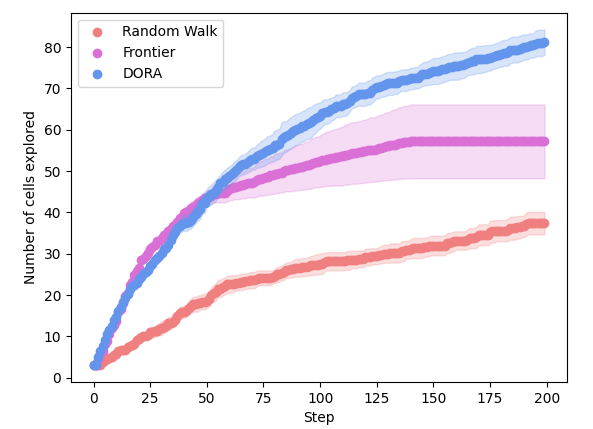
\includegraphics[width=\textwidth]{figures/dora_explorer/explored_real.png}
        \caption{N=5 physical robots}
        \label{results:cells_explored_physical}
    \end{subfigure}
    \caption[DORA cell exploration performance]{Performance comparison of \ac{DORA}, \ac{FBE} and random walk for number of explored cells over time.  Fig. \ref{results:explored10}, \ref{results:explored15}, \ref{results:explored20} are for simulations; Fig. \ref{results:cells_explored_physical} is for physical experiments.}
    \label{results:dora_explored}
\end{figure*}

Where \ac{DORA} truly shows its worth is in Fig. \ref{results:dora_active}, in which the number of active robots over time is presented. Indeed, in every experiment scenario, \ac{DORA} experienced far fewer robot failures than both benchmark algorithms. As for terrain coverage, \ac{DORA}'s performance improves with respect to the other algorithms as the number of robots involved increases. This further shows our algorithm's scalability.

\begin{figure*}
    \centering
    \begin{subfigure}{0.45\textwidth}
        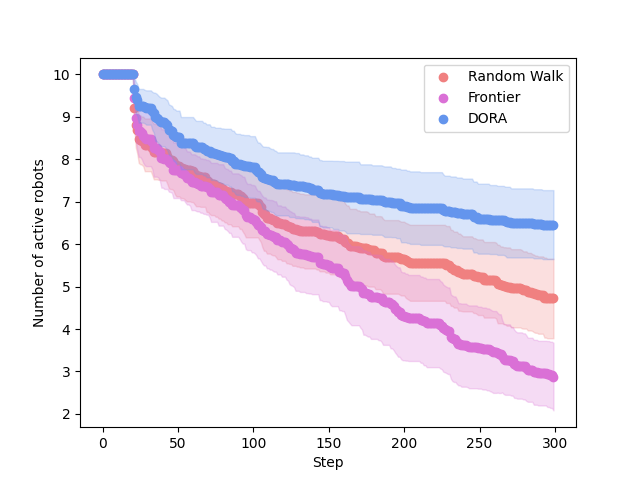
\includegraphics[width=\textwidth]{figures/dora_explorer/activerobots_10.png}
        \caption{N=10 robots}
        \label{results:failures10}
    \end{subfigure}
    \begin{subfigure}{0.45\textwidth}
        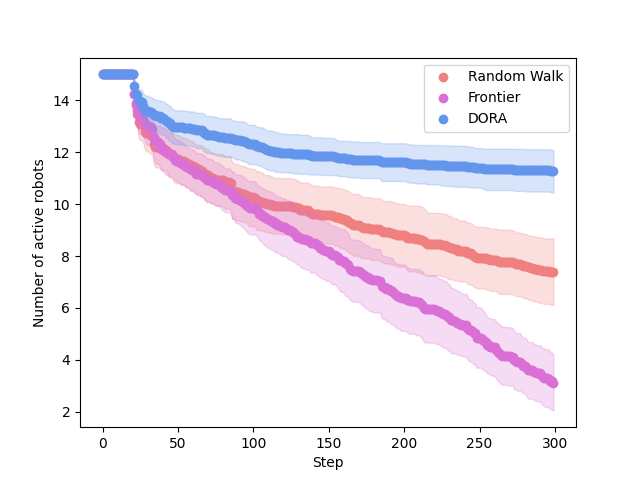
\includegraphics[width=\textwidth]{figures/dora_explorer/activerobots_15.png}
        \caption{N=15 robots}
        \label{results:failures15}
    \end{subfigure}
    \begin{subfigure}{0.45\textwidth}
        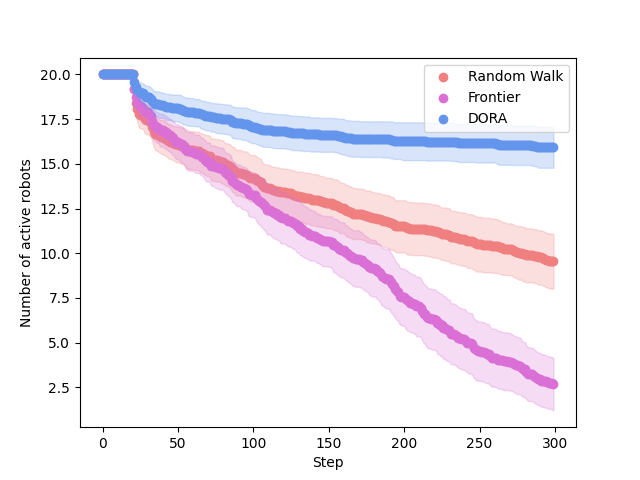
\includegraphics[width=\textwidth]{figures/dora_explorer/activerobots_20.png}
        \caption{N=20 robots}
        \label{results:failures20}
    \end{subfigure}
    \begin{subfigure}{0.45\textwidth}
        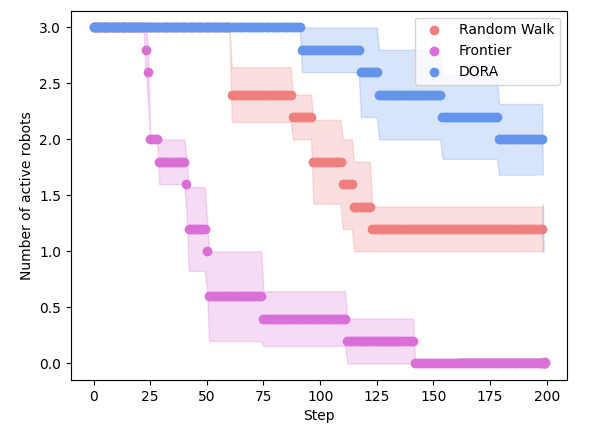
\includegraphics[width=\textwidth]{figures/dora_explorer/activerobots_real.png}
        \caption{N=5 physical robots}
        \label{results:active_robots_physical}
    \end{subfigure}
    \caption[DORA survival performance]{Performance comparison of \ac{DORA}, \ac{FBE} and random walk for number of active robots over time. Fig. \ref{results:failures10}, \ref{results:failures15}, \ref{results:failures20} are for simulations; Fig. \ref{results:active_robots_physical} is for physical experiments.} 
    \label{results:dora_active}
\end{figure*}

Intuition for how \ac{DORA} results from Fig.\ref{results:dora_explored} and Fig. \ref{results:dora_active} are related can be gained by observing Fig. \ref{results:belief}. Whereas \ac{FBE} visited the areas around the radiation sources (as can be seen by the cells with a high radiation level), \ac{DORA} avoided them. This results in a slightly lower exploration coverage, but in a much lower failure rate.

\begin{figure*}
    \centering
    \begin{subfigure}{0.45\textwidth}
        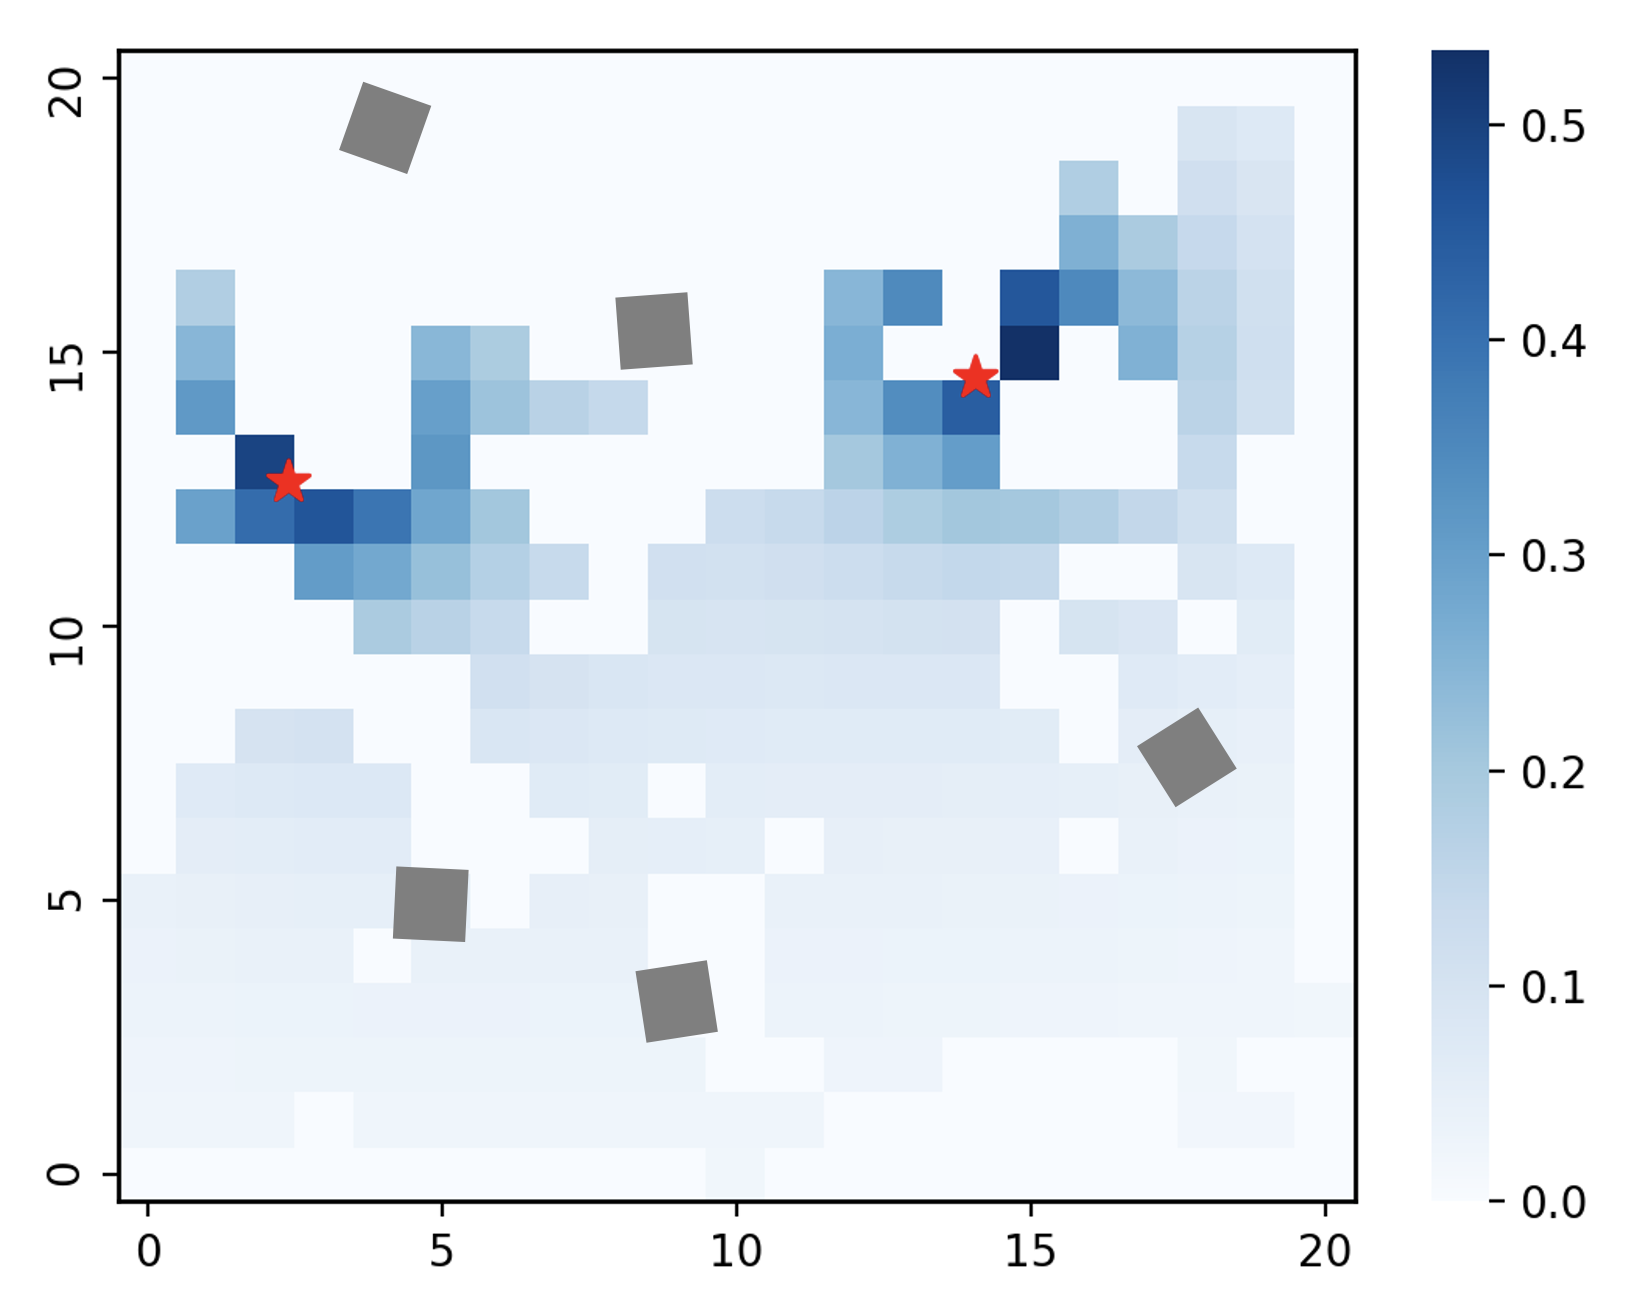
\includegraphics[width=\textwidth]{figures/dora_explorer/heatmap_random.png}
        \caption{Random walk}
        \label{results:beliefrandom}
    \end{subfigure}
    \begin{subfigure}{0.45\textwidth}
        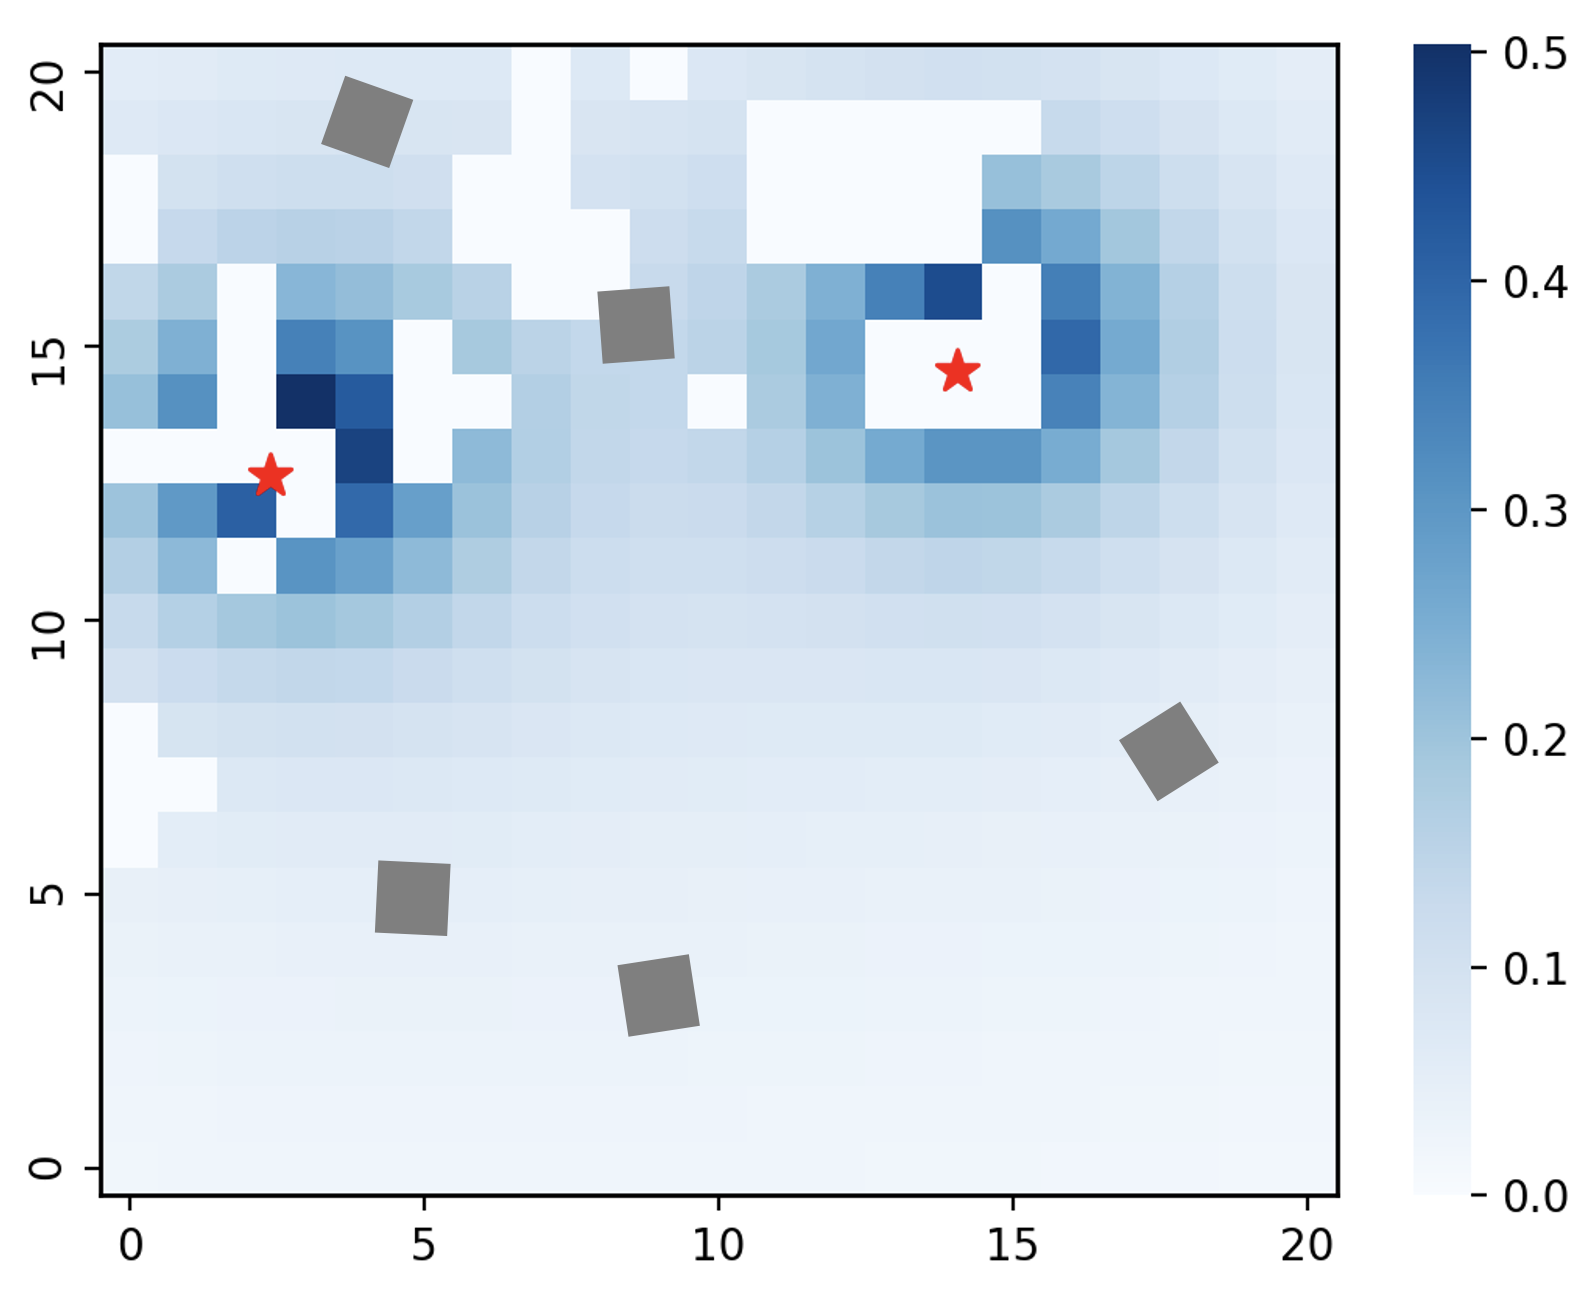
\includegraphics[width=\textwidth]{figures/dora_explorer/heatmap_frontier.png}
        \caption{\ac{FBE}}
        \label{results:belieffrontier}
    \end{subfigure}
    \begin{subfigure}{0.45\textwidth}
        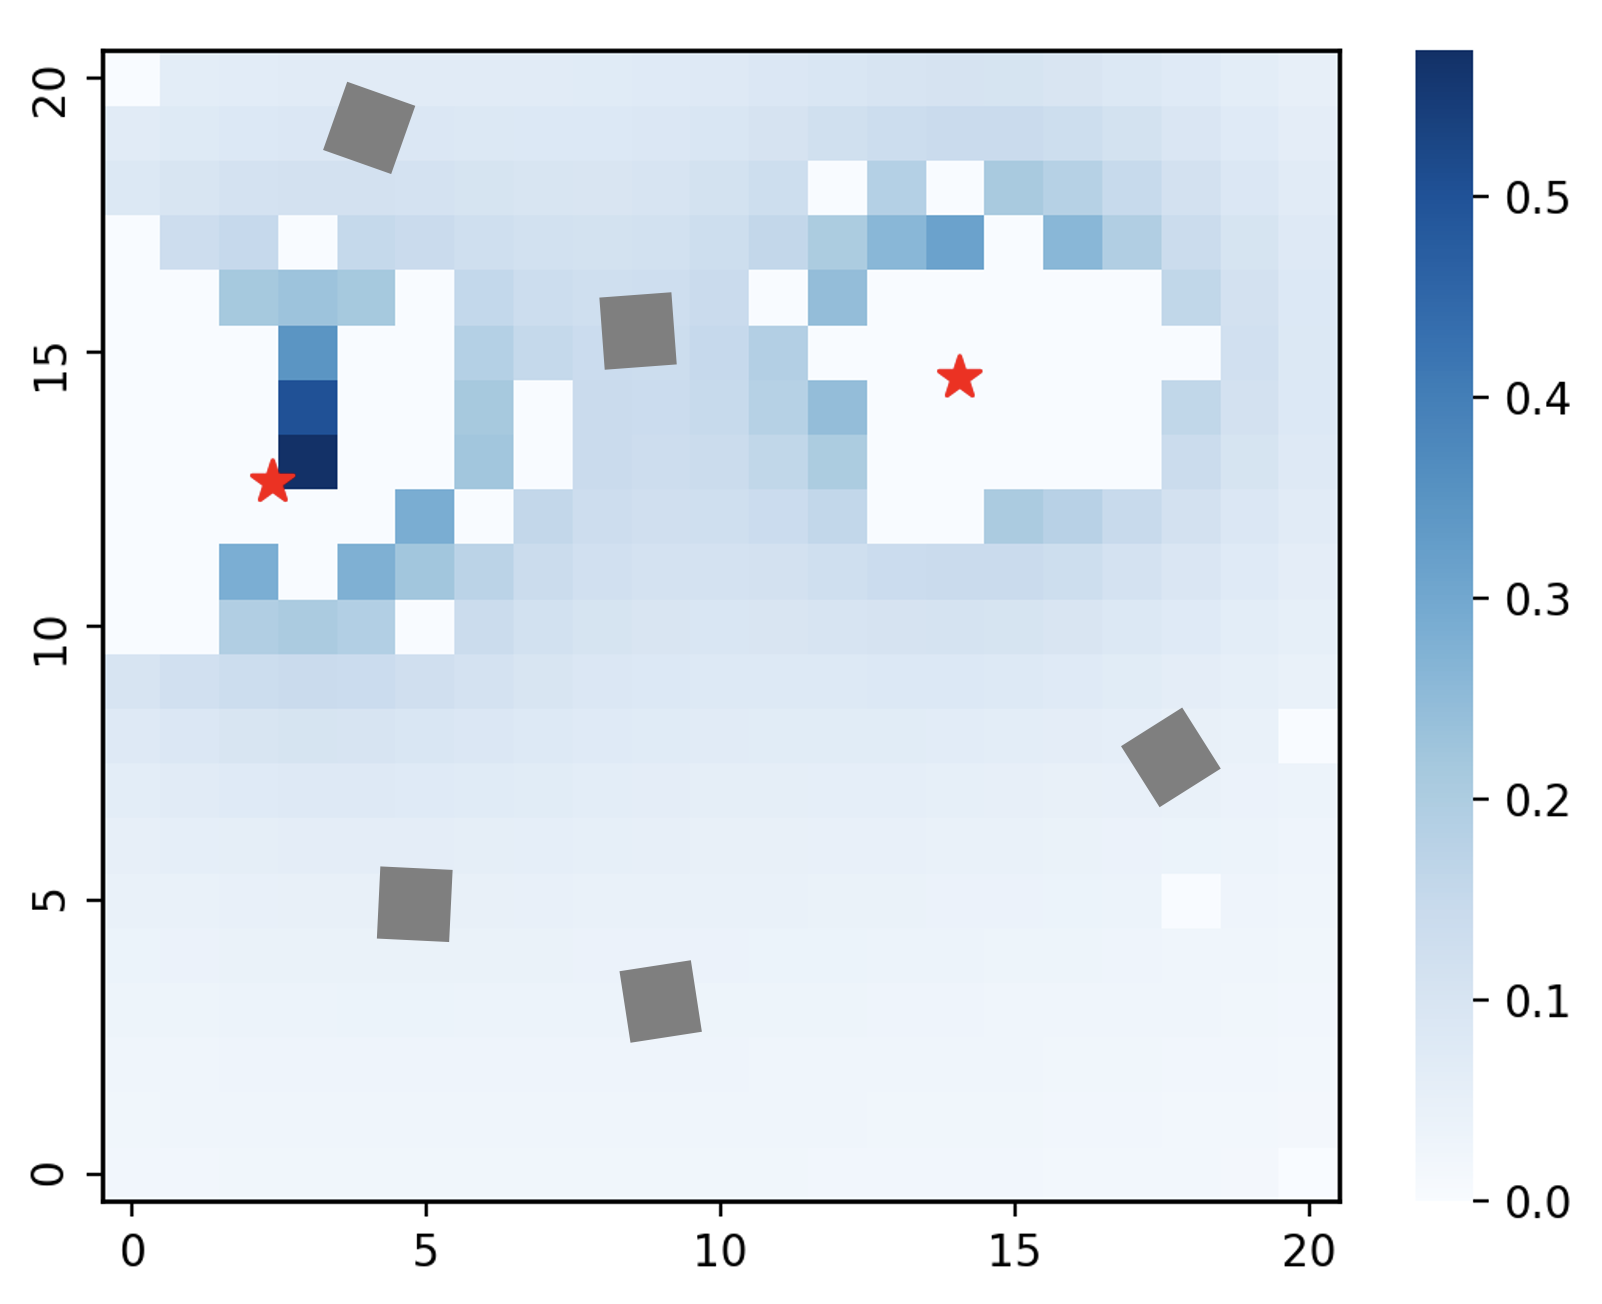
\includegraphics[width=\textwidth]{figures/dora_explorer/heatmap_dora.png}
        \caption{\ac{DORA}}
        \label{results:beliefdora}
    \end{subfigure}
    \caption[DORA radiation belief maps]{Examples of radiation belief maps of the 20x20m environment for each exploration algorithm of one specific simulation. Blank cells are unvisited areas, red stars are the point radiation sources and grey squares are the randomly generated obstacles.}
    \label{results:belief}
\end{figure*}

In Fig. \ref{results:communicationCosts}, we can see the amount of data exchanged by robots in the simulations conducted with \ac{DORA} and \ac{FBE}. The takeaway is that \ac{DORA} outperforms \ac{FBE} by a significant margin for this metric, and that communication costs are aligned with the theoretical values from \ref{dora_system_model}. This metric was not calculated for the random walk algorithm as it does not require any coordination nor communication. It was not measured in physical experiments.

\begin{figure}[htbp]
    \centering
    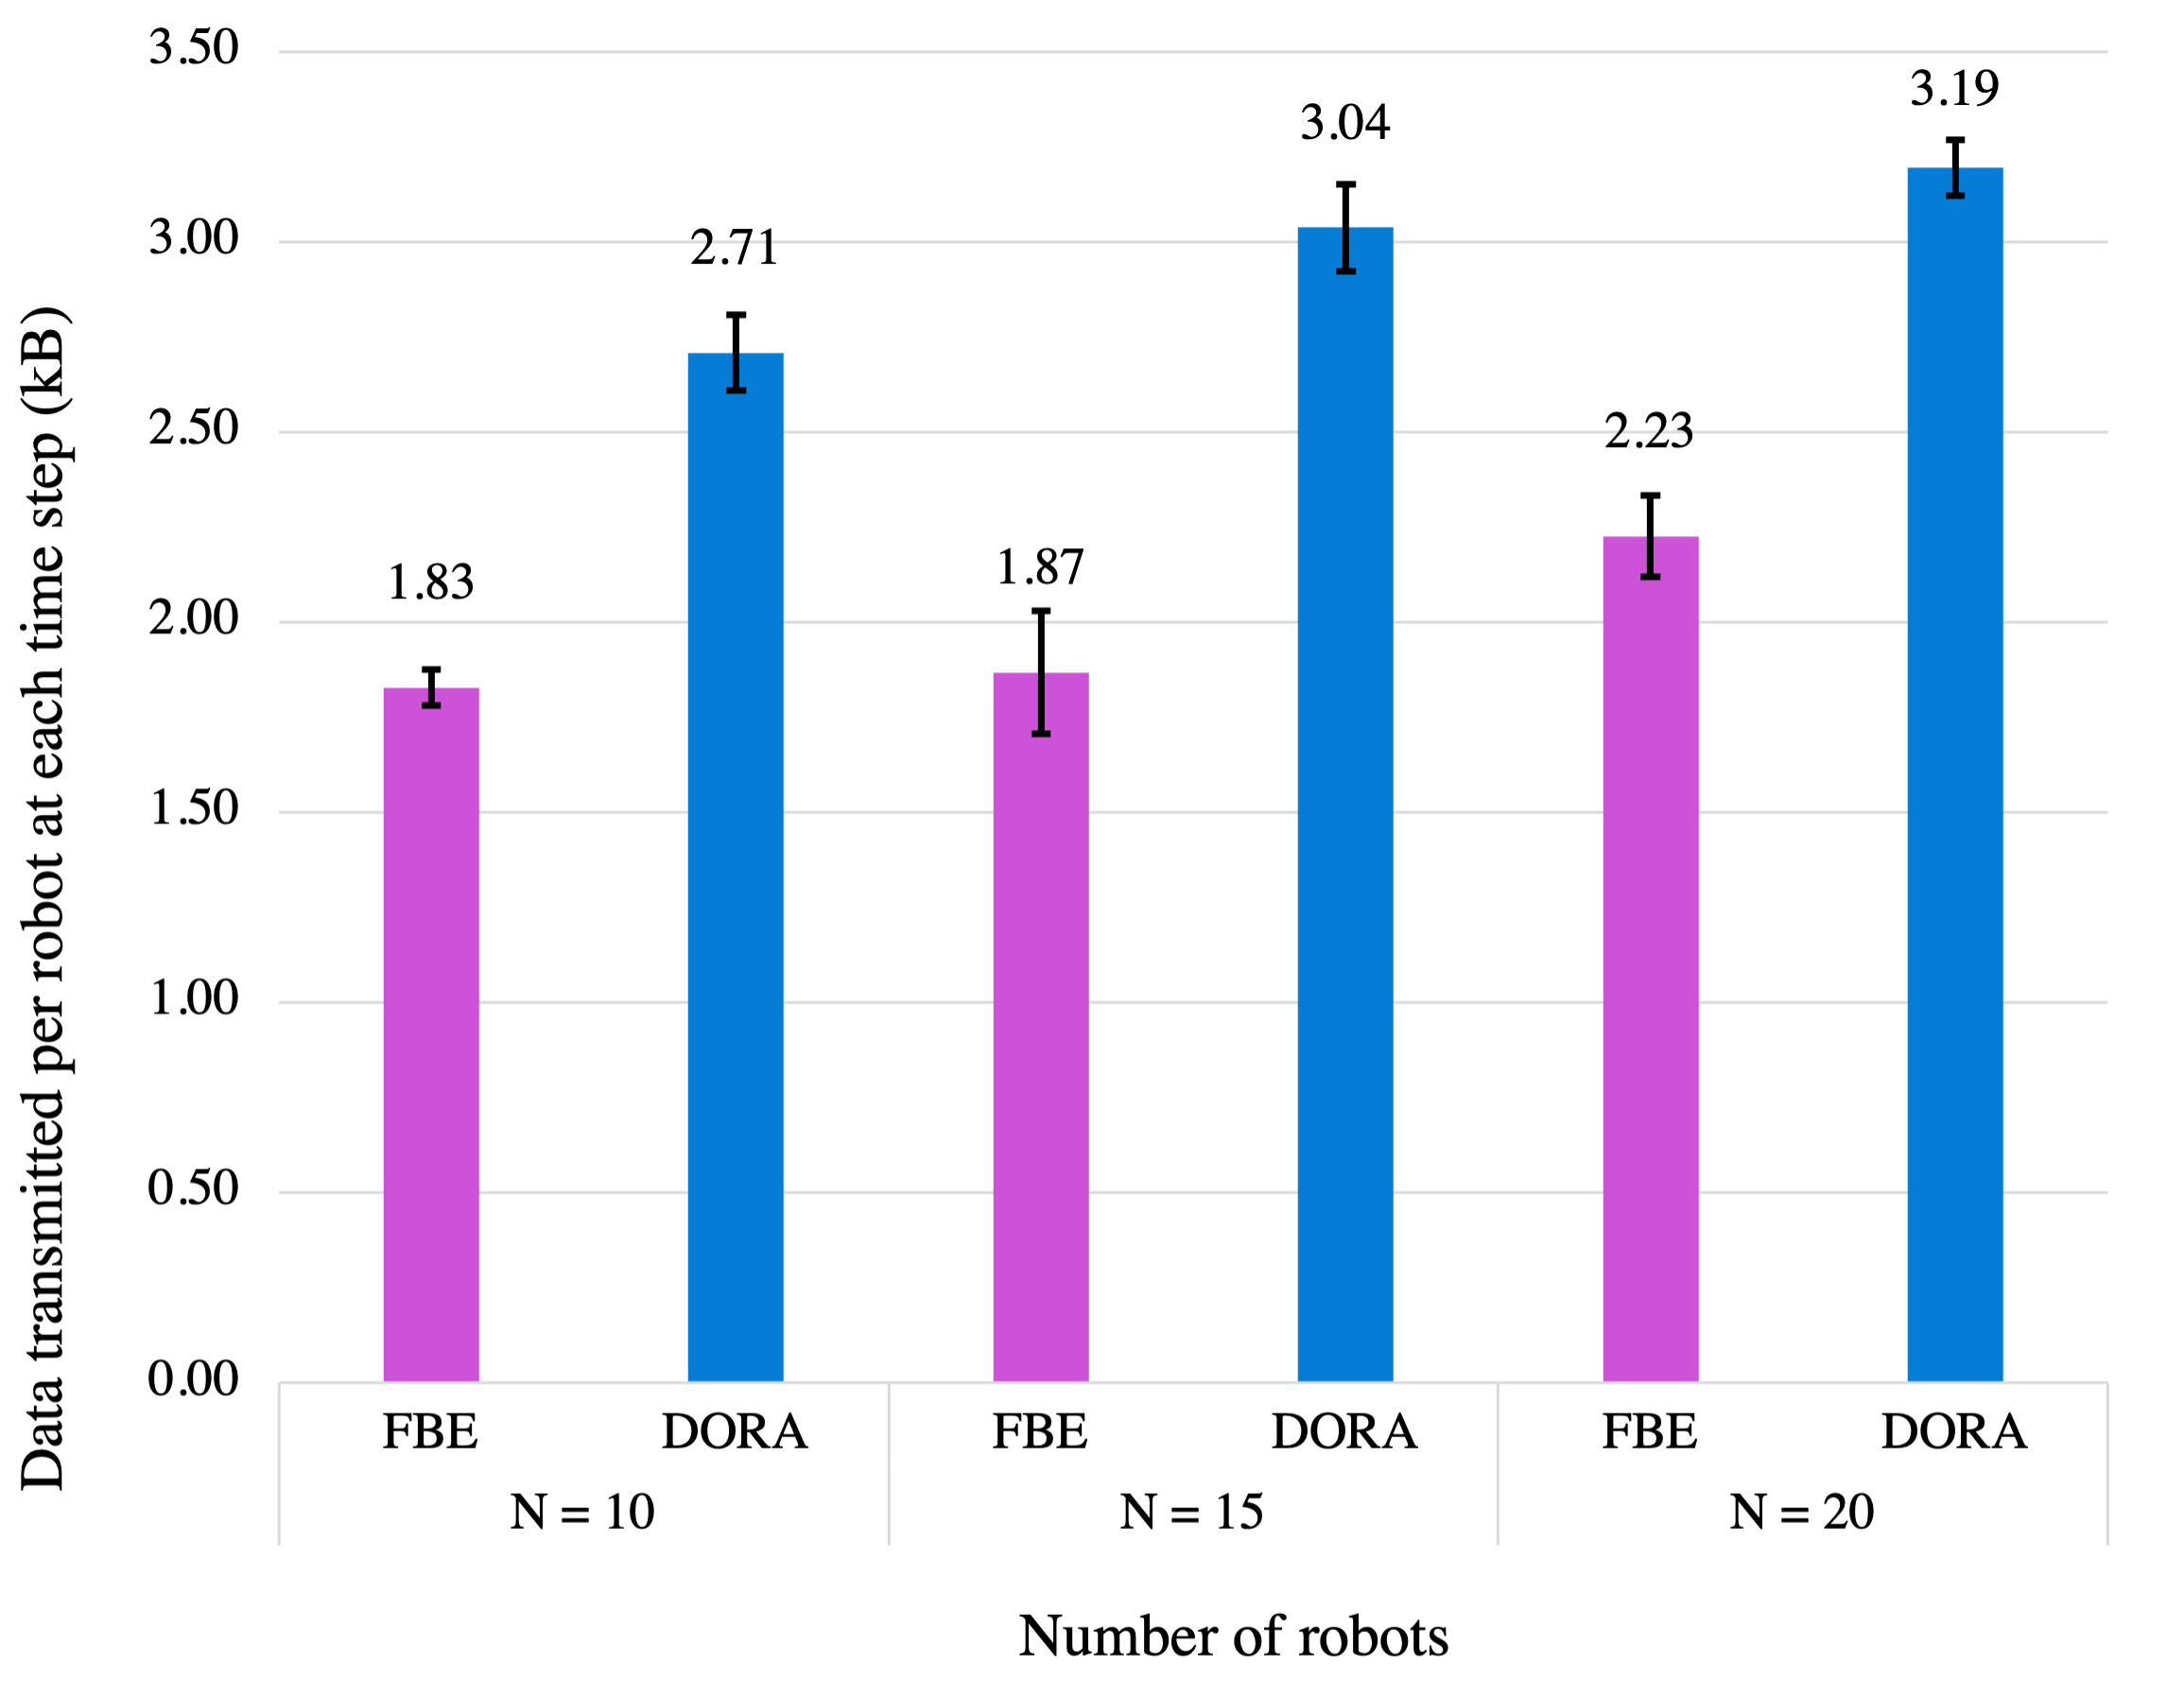
\includegraphics[width=0.9\textwidth]{figures/dora_explorer/communication.png}
    \caption[DORA communication costs]{Communication costs for \ac{DORA} and \ac{FBE}}
    \label{results:communicationCosts}
\end{figure}

\FloatBarrier

\section{Conclusion}
\ac{DORA} Explorer is a lightweight risk-aware exploration algorithm. It minimizes the risk to which robots expose themselves to allow them to maximize the amount of explored terrain. By leveraging \ac{DBM}s it outperforms non-coordinated solutions. Indeed, it succeeds in considerably reducing the likeliness of robot failures while keeping similar ground coverage performance compared to other solutions proposed in the literature. \ac{DORA} also showed good scalability thanks to its low communication costs. It also showed applicability to real world scenarios through experiments with physical robots.

In future work, it could be interesting to modify \ac{DORA} to allow time-varying risk-tolerance thresholds. Additionally, this work assumed that the risk associated with the environment can be measured by the robots' sensors, which is not always the case. To account for this issue, risk belief maps could be constructed using the previous failures of the agents to infer the presence of danger.
